We first motivate the need for another architectural description language, then we present the fundamental concepts necessary for such a language. We focus on three concepts: clock models, channel \& buffer models, and fault models.

\subsection{Why Another ADL?}

With the numerous architectural description languages (ADLs) and accompanying
tools available (see Section~\ref{ssec:modeling}), we must ask is
is, \emph{"Why another ADL?"}.
We are focused on the correct specification and synthesis of distributed systems
and the formal verification and validation of distributed system protocols.  A
key research goal is to provide a specification framework that encompasses a
suitable level of abstraction to allow for the efficient behavioral
specification of distributed fault-tolerant protocols.  Additionally, we desire
for protocol specifications to exist within the larger context of the system
architecture and anticipated fault models.

Currently, AADL is one of the most mature ADLs, yet, in our work to date we have
found that expressing the details such of protocols with AADL is non-trivial,
with certain aspects not yet possible. such as behaviours that are not
compatible with the underlying AADL dispatch semantics.

%% Although AADL may evolve
%% to capture the required semantics, the pace of change that can be accommodated
%% with standardized languagesis another concern.  Only now, two years after the
%% research completed, are the some of the changes identified by the
%% AFCS~\cite{afcs} research are getting addressed by the AADL working
%% committee. Rather, than pace our research with such timescales, we feel that
%% there may be greater benefit in identifying the needs through our targeting of
%% AADL as an implementation language.

A second goal is integrating the models of faults and behavior.  Once again,
this is an area where current ADLs are lacking. For example, in
AADL, the integration of the behavioral and error annexes is not mature, and
hence cross-annex formal semantics and linkages are not defined.  In addition,
although the LIMA language (see Section~\ref{ssec:modeling}) incorporates provisions
for integrated specification, the level of abstraction is more
cumbersome than it should be.  This is another area where our
synthesis strategy to an intermediate ADL may be beneficial. For example, using
our approach, we may be able to efficiently synthesize LIMA models for formal
analyses, where such models may too expensive to develop by hand.

The final intent is to link the formal assurance argument within the ADSL work
flow. Once again, this is an area where the current ADLs continue to develop;
the recent work with AADL and RESOLUTE~\cite{gacek2014resolute} looks
promising.

In summary, there exist no ADLs that allow the efficient
specification and refinement of system models and protocol specification. Our
hope is that it will be more efficient and lighteweight. That said, where formal
semantics exist for intermediate ADLs, our ADSL can target them.


%% However, rather than be limited by the current capabilities, our
%% intent is that ADSL can link to what works and where necessary develop new
%% capabilities to address areas of identified need.


%% Finally, given the ADSL's functional host langauge (see
%% Section~\ref{sec:adsl}), we further anticipate great benefits as we leverage
%% test generation frameworks such as QuickCheck~\cite{monadic} to the
%% architectural specification, especially if such generation can be aligned with
%% the formal fault model.

%% \subsection{ADSL Approach}
%% The core of the technical approach is that we are able to synthesize both formal
%% models and implementation models directly from the ADSL specification in
%% our ADSL workbench. In order for the ADSL to be useful, it has to be expressive
%% enough with sufficient variety of primitives to cover a breadth of models
%% supporting varying networks, architectures, and systems as covered by the case
%% studies described in Section~\ref{sec:case-studies}. The ADSL must also be rich
%% enough to describe in sufficient depth each case study to go from high level
%% architecture models (e.g., AADL) to all implementation level details and models.

%% \lee{This needs to be fleshed out}

%% Currently in our research, we have restricted ourselves to primarily focusing on
%% developing SAL~\cite{SRI:SAL} formal models and AADL architectural models as targets
%% to be synthesized from our ADSL specification.  Our strategy is two fold.

%% First, we take a \emph{bottom-up} approach of describing some basic elements and
%% building blocks that must be captured in our ADSL
%% (Section~\ref{subsec:ADSL_Elements}). The idea is that
%% then we will have to flesh out enough of these basic building blocks and build
%% layers of abstractions from them, composing them systematically (potentially
%% hierarchically) and constructing larger models of the systems of interest based
%% on our case studies from them.

%% Second, we also take a \emph{top-down} approach of describing the targets for
%% the three case studies in Sections~\ref{subsec:ADSL_CaseStudy_1}
%% and~\ref{subsec:ADSL_CaseStudy_3} that help us drill down further and narrow
%% some of the ADSL primitives that definitely must be developed.

%% With both the approaches described above, we have gained valuable insights
%% and intend to incorporate the lessons learned into the ADSL and corresponding
%% synthesis framework within the ADSL workbench. At the time of writing,
%% we do not yet have exact and full ADSL specifications with appropriate
%% abstractions nor have we completed all of the actual
%% synthesis for targets for the given case studies (though we have the synthesis
%% framework itself) . We are still in the process of researching the right levels
%% of abstractions in the ADSL framework and the costs/benefits of synthesis with
%% respect to the scalability of the formal models so synthesized in terms of its
%% ability to prove different properties of interest and efficiency of synthesis to
%% implementation models.

%% So at the time of this report we simply outline the progress we've made thus far
%% and also describe some of thoughts that should feed into the development of the
%% ADSL specifications and ADSL development in years II and III.


\subsection{ADSL Concepts}
\label{subsec:ADSL_Elements}

The three fundamental concepts we present are clocks, channels \& buffers, and faults to describe real-time distributed systems. We describe each in turn.

As we describe the following, we present the concepts based on the notion of an \emph{atom}. An atom is a hierarchical state-machine. An atom can represent a node in a distributed system, but we also allow for the existence of a \emph{sub-atom}, that is a sub-component of a node. Atoms allow us to decompose specifications. We call a sub-atom's encompassing atom the sub-atom's \emph{parent}.

\subsubsection{Clock Model}
\label{subsubsec:clock_model}

\begin{figure}[h!]
\centering
\caption{Clocked Atom Model}
 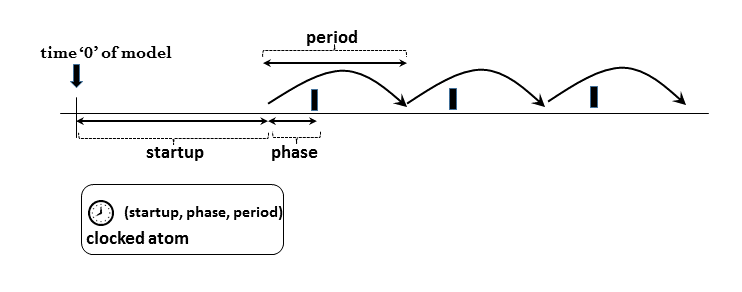
\includegraphics[width=0.75\textwidth]{figures/clocked_atom.png} 
\label{fig:clock_atom_model}
\end{figure}

In modeling distributed systems, we must often assign clocks to atoms to measure its notion of the passage of time. The notion of clocked nodes are \emph{periodic} processes or tasks.  A clocked atom is defined by a tuple of three parameters as shown in Figure~\ref{fig:clock_atom_model}:
\begin{itemize}
\item {\it startup} which indicates the duration of time elapsed from time $0$ when the clock starts ticking away i.e. initialized \emph{start up delay} for the clock. Note that this startup can span multiple periods potentially. $startup \geq 0$
\item {\it phase} is the \emph{offset} within the period when the task/process is executed periodically. $0 \leq phase < period$
\item {\it period} is the periodicity of the task i.e. inverse of the frequency of the task.
\end{itemize}

All \emph{derived} clocked atoms or \emph{sub-atoms} from parent have
synchronous clocks with respect to the parent clock. This means, as shown in
figure \ref{fig:sync_clock_atom_model}, the $startup$ of the sub-atoms are
identical to their parent and their clocks are initialized identical to their
parent.  As shown in the figure both $atom1$ and $atom2$ derived from $atom$
have identical $startup$ parameter. Also the \emph{derived atoms's phases are
additive} Thus $atom1$ has an effective phase $phase+phase1$ from start of
period and $atom2$ has an effective phase $phase+phase2$ from the start of the
period. Also derived atoms period are harmonic with respect to the parent and
at equal or slower rate. For example in the figure $period1 = period$ while
$period2 = 2 \times period$. Thus atom and sub-atom relationships can be used
to model synchronous system whereby all distributed system nodes which are
synchronous with each other can be modeled as sub-atoms with clocks under a
single parent atom with a ``notional'' clock for the whole system. Similarly
ARINC~653~\cite{arinc653} partitions or tasks within a single node can be
modeled as sub-atoms with a single parent atom.

\begin{figure}[h!]
\centering
\caption{Synchronous Derived Atom Clock Model}
 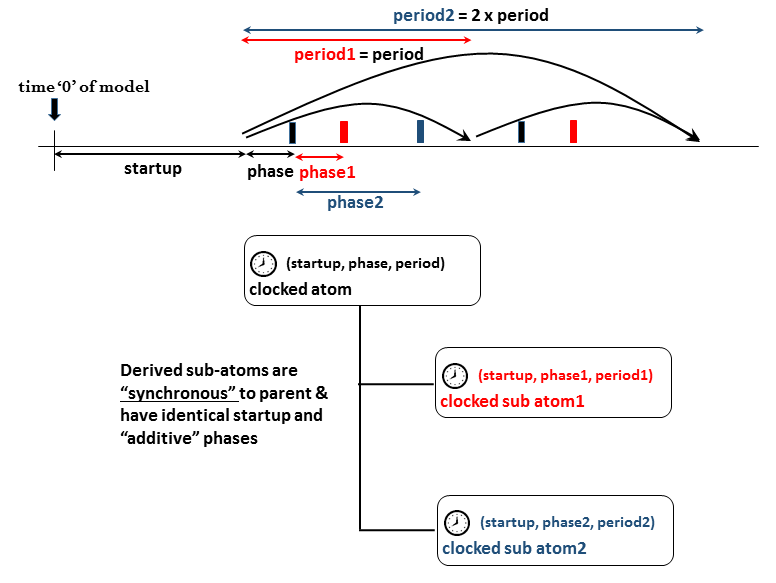
\includegraphics[width=0.75\textwidth]{figures/sync_clocked_atom.png}
\label{fig:sync_clock_atom_model}
\end{figure}

\begin{figure}[h!]
\centering
\caption{Asynchronous Peer-to-Peer Atom Clock Model}
 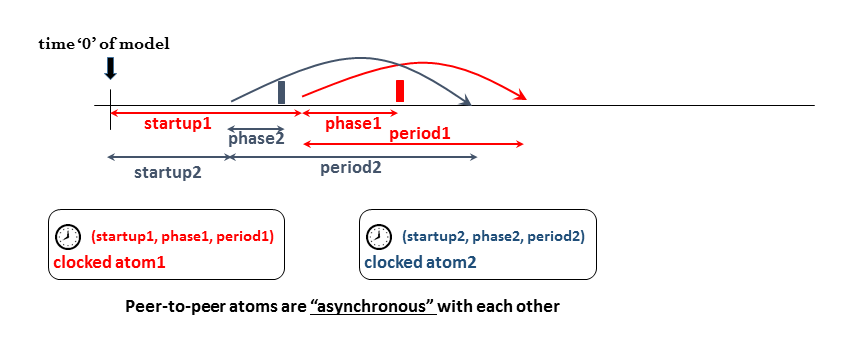
\includegraphics[width=0.75\textwidth]{figures/async_clocked_atom.png}
\label{fig:async_clock_atom_model}
\end{figure}

On the other hand, as shown in Figure~\ref{fig:async_clock_atom_model}, two peer clocked atoms at the top level are considered \emph{asynchronous} with each other. As shown in the figure, their individual $startup$, $phase$, and $period$ for their respective clocks have no relationship with each other.

During verification, it can be useful to allow startup times, periods, and phases to be nondeterministic (without violating the constraints above) to verify timing properties about the system under abstract constraints. For example, one might state timing constraints and verify that the system implements time-triggered behavior~\cite{fmcad07}. During C simulation, however, these timing values must take on constant values.


\subsubsection{Channel \& Buffer Model}
\label{subsubsec:channel_buffer_model}


System designers typically have to contend with managing resource constraints across networked systems. There are two high level resources they need to balance: (i) platform resources like CPU utilization (time) and memory (space) vs (ii) network resources like bandwidth/link usage manifesting as transport/channel delay (time) and network card memory/channel buffers (space). Since both platform and network resources along both time and space dimensions are all finite, optimizing along just one of those resources and/or dimension at the cost of the other is not a viable option. Correct characterization of computation time, communication time (channels delay) and associated buffers (memory at platform or network) at every node is a critical element of the ADSL as it lays the foundation for accurate modeling of platform and network resources in the system.  We show the time and space attributes of network resources in terms of channel and buffer models in Figure~\ref{fig:channel_buffer}. 

A channel is modeled as \emph{unidirectional} flow of message $M$ from a transmitter Node $T$ to multiple receiver Nodes $R_1,R_2,...,R_n$ with corresponding channel delays $D_1,D_2,...,D_n$. Channel delays are all different because there may be different transport paths from transmitter to the different receivers. Channel delays are a function of the size of message $M$, the network bandwidth/link rates, the propagation time (wire length) and the number of intermediate relays between transmitter and the receiver. Thus a message transmitted on to the channel at time $T_1$ from Node $T$ is received at each of the receiver from the channel at times $T_1+D_1, T_1+D_2, T_1+D_3,...,T_1+D_n$ respectively. Note that \emph{unicast}, \emph{multicast} and \emph{broadcast} are all supported with this model of channel.

Also note that as shown in the Figure~\ref{fig:channel_buffer}, there is string of \emph{producing} processes and \emph{consuming} processes in the model and this must correctly identified in-order and in-sequence to get the modeling of the buffer (e.g. overflow or size) correct and this is described next. For example, in Node $T$, there is some platform application that is producing a message (possibly from a computation process) and this produced message is stored in the channel buffer (network card memory). The network card in Node $T$ subsequently reads from its own memory (channel buffer) and produces (transmits) the message on to the channel. 

The process is then reversed at the receiver. The receiver network card consumes the message from the channel and stores the message locally into its own channel buffer (network card memory). Then either the network card reads from its channel buffer and pushes the message to consuming platform process OR the consuming platform process reads from the channel buffer and then finally processes the message as it sees fit (possibly sent to a computation process).

Since Produce/Transmission at $T$ and Consume/Reception(s) at $R$ can be
triggered by ``independent'' clocked atoms (described in section
\ref{subsubsec:clock_model}) at $T$ and $R(s)$, the buffer model is critical
to manage the differences in rates and timing between production and
consumption. Once the processes are correctly modeled as stated above, then we
identify two types of channel buffers at either the transmitter or at the
receivers:

\begin{itemize}
\item \emph{Queuing}: First-in-First-Out (FIFO) Order i.e. messages are taken out of the queue in the order in which data was produced into it.  The maximum size of the queue is also specified as $k$. If messages are not consumed at fast enough rate compared to rate at which message are produced into the buffer and once the queue is already filled with ``k'' messages yet to be consumed, then produced message(s) are dropped. 

\item \emph{Sampling}: New message produced overwrites old message if not consumed.

\end{itemize}


\begin{figure}
\begin{center}
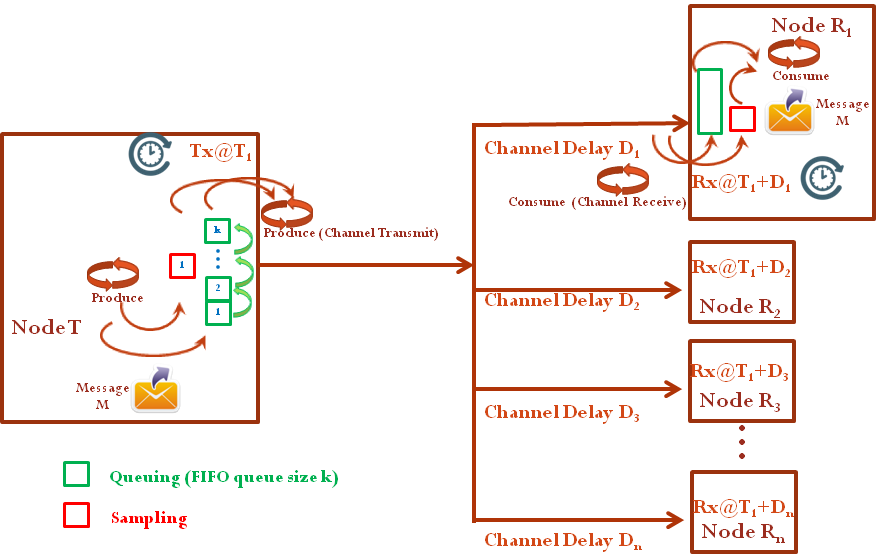
\includegraphics[width=0.8\textwidth]{figures/channel_buffer.png}
\caption{Channel and Buffer Models}
\label{fig:channel_buffer}
\end{center}
\end{figure}

\subsubsection{Fault Model}

The ability to model and specify fault models is a  significant capability
of the proposed ADSL. Faults can occur at different levels of abstraction, and an ADSL should have the capability of specifying and reasoning about faults at the different levels as well as mapping between them.

In particular, we distinguish between local and global faults.
Following the taxonomy of Avizienis~\emph{et~al.}~\cite{taxonomy},
we refer to faults that occur locally in any component, such as a node or channel, as being modeled as \emph{local faults}. Some examples of
local faults are:
\begin{itemize}
  \item Omission (message loss)
  \item Commission (babbling)
  \item Untimely (late, early, sequence violation etc.)
  \item Invalid value (semantic, syntactic,..)
  \item Invalid protocol behavior (e.g., failure of fault handling of detection,
protection etc).
\end{itemize}

On the other hand, \emph{global faults} are based on relationships between
two or more components (i.e., nodes or channels) at the system level. Examples of system
faults include \emph{symmetric} and \emph{asymmetric} transmission faults~\cite{Tha88:RDSS}. Global faults
may be dependent on the expected of degree of consensus~\cite{lynch}, which in itself is
tied to the application's sensitiveness to disagreements, independence assumptions, or degree of maliciousness (e.g. assumptions on how coordinated two or more nodes can be in triggering failures). Global faults based on relationships between two or more components can cause interactive consistency (consensus violations) and Byzantine issues at the system level.


\begin{figure}
\begin{center}
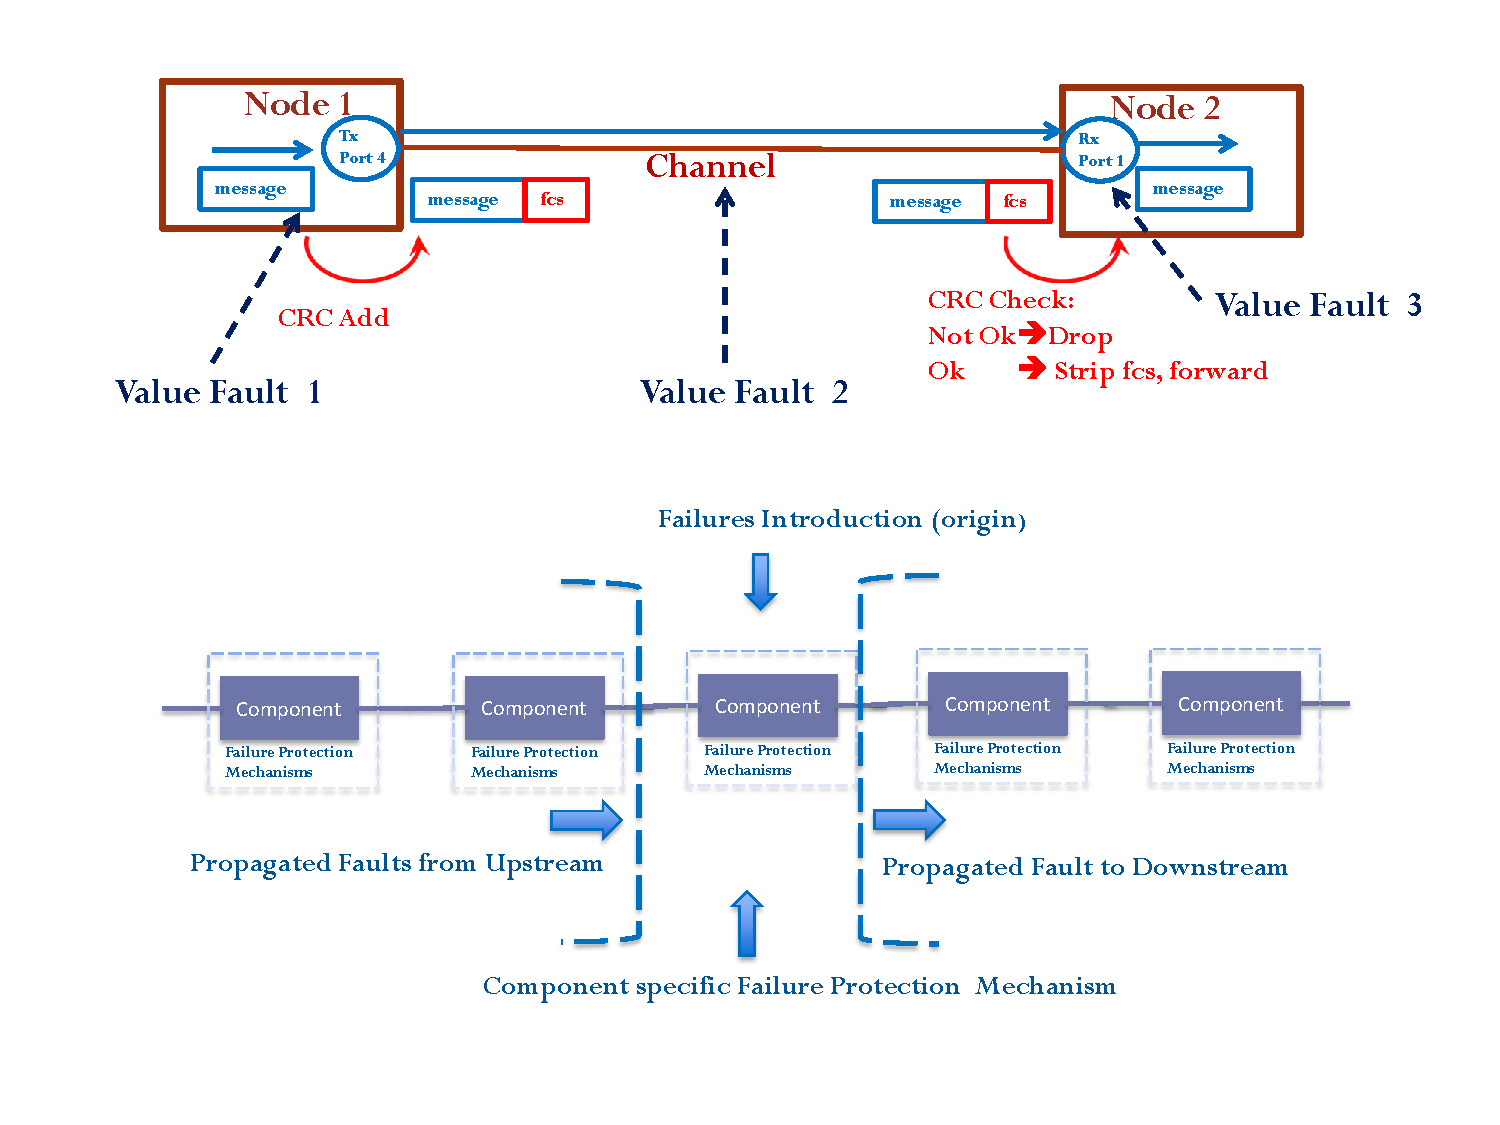
\includegraphics[width=0.8\textwidth]{figures/fault_propagation.pdf}
\caption{Fault Propagation}
\label{fig:fault_propagation}
\end{center}
\end{figure}

Finally, we wish to also characterize fault
propagation through the networked system, originating in some component and
propagating from one component to another, as shown in the bottom of
Figure~\ref{fig:fault_propagation}. Faults introduced/propagated from upstream
components transform to other faults based on protection mechanisms built
into
each component (e.g., a commission fault transforms into an omission fault
if a
bandwidth check is implemented as protection mechanism in a component)~\cite{theory}.

To illustrate this in a concrete example, refer to a cyclic redundant check
(CRC) protection behavior illustrated at the top of
Figure~\ref{fig:fault_propagation}. Nominally in a fault-free operation,
$Node_1$ adds a CRC to a message when it transmits over the channel, and
when
$Node_2$ receives the message, it does a CRC check by comparing the re-computed
CRC
with the frame check sequence (FCS). If the check fails, the message is dropped,
and if the check
passes, then the FCS is stripped and the message is forwarded. Note that
fault-free
(nominal) behavior of a CRC check at the receiver is that (i) a good message
is
never dropped incorrectly, (ii) a bad (corrupt) message is dropped with high
probability, and (iii) there is also a small finite probability that a bad
message escapes detection and drop (e.g. based on efficacy of CRC 32 etc.)~\cite{crc}.

Value Fault~1 in Figure~\ref{fig:fault_propagation} introduced in the node
either at the indicated point or introduced upstream before that point and
propagated until that point will also continue to propagate downstream and
CRC
offers no protection. This is because the FCS is added on an already corrupted
message. Value Fault~2 introduced in the channel will be protected by CRC
(modulo the CRC's efficacy). Further Value Fault~2 will transform to Omissive Fault downstream due the CRC protection. 
Value Fault~3 introduced in $Node_2$ at that
point will propagate downstream as it is after CRC protection.

The idea then is to capture a fault transformation function in every
component
node/link based on behavior fault-protection schemes available at that component;
e.g., a value fault transforms to an omissive fault for CRC protection. 
These will be
specified in a static manner at every component. This way, both horizontal
propagation of faults (CRC example) and vertical propagation of faults
(e.g., self-checking hardware) can be modeled as a component embedded
in another
component) can be captured in an ADSL framework.


